% Options for packages loaded elsewhere
\PassOptionsToPackage{unicode}{hyperref}
\PassOptionsToPackage{hyphens}{url}
%
\documentclass[
]{book}
\usepackage{amsmath,amssymb}
\usepackage{lmodern}
\usepackage{iftex}
\ifPDFTeX
  \usepackage[T1]{fontenc}
  \usepackage[utf8]{inputenc}
  \usepackage{textcomp} % provide euro and other symbols
\else % if luatex or xetex
  \usepackage{unicode-math}
  \defaultfontfeatures{Scale=MatchLowercase}
  \defaultfontfeatures[\rmfamily]{Ligatures=TeX,Scale=1}
\fi
% Use upquote if available, for straight quotes in verbatim environments
\IfFileExists{upquote.sty}{\usepackage{upquote}}{}
\IfFileExists{microtype.sty}{% use microtype if available
  \usepackage[]{microtype}
  \UseMicrotypeSet[protrusion]{basicmath} % disable protrusion for tt fonts
}{}
\makeatletter
\@ifundefined{KOMAClassName}{% if non-KOMA class
  \IfFileExists{parskip.sty}{%
    \usepackage{parskip}
  }{% else
    \setlength{\parindent}{0pt}
    \setlength{\parskip}{6pt plus 2pt minus 1pt}}
}{% if KOMA class
  \KOMAoptions{parskip=half}}
\makeatother
\usepackage{xcolor}
\usepackage{color}
\usepackage{fancyvrb}
\newcommand{\VerbBar}{|}
\newcommand{\VERB}{\Verb[commandchars=\\\{\}]}
\DefineVerbatimEnvironment{Highlighting}{Verbatim}{commandchars=\\\{\}}
% Add ',fontsize=\small' for more characters per line
\usepackage{framed}
\definecolor{shadecolor}{RGB}{248,248,248}
\newenvironment{Shaded}{\begin{snugshade}}{\end{snugshade}}
\newcommand{\AlertTok}[1]{\textcolor[rgb]{0.94,0.16,0.16}{#1}}
\newcommand{\AnnotationTok}[1]{\textcolor[rgb]{0.56,0.35,0.01}{\textbf{\textit{#1}}}}
\newcommand{\AttributeTok}[1]{\textcolor[rgb]{0.77,0.63,0.00}{#1}}
\newcommand{\BaseNTok}[1]{\textcolor[rgb]{0.00,0.00,0.81}{#1}}
\newcommand{\BuiltInTok}[1]{#1}
\newcommand{\CharTok}[1]{\textcolor[rgb]{0.31,0.60,0.02}{#1}}
\newcommand{\CommentTok}[1]{\textcolor[rgb]{0.56,0.35,0.01}{\textit{#1}}}
\newcommand{\CommentVarTok}[1]{\textcolor[rgb]{0.56,0.35,0.01}{\textbf{\textit{#1}}}}
\newcommand{\ConstantTok}[1]{\textcolor[rgb]{0.00,0.00,0.00}{#1}}
\newcommand{\ControlFlowTok}[1]{\textcolor[rgb]{0.13,0.29,0.53}{\textbf{#1}}}
\newcommand{\DataTypeTok}[1]{\textcolor[rgb]{0.13,0.29,0.53}{#1}}
\newcommand{\DecValTok}[1]{\textcolor[rgb]{0.00,0.00,0.81}{#1}}
\newcommand{\DocumentationTok}[1]{\textcolor[rgb]{0.56,0.35,0.01}{\textbf{\textit{#1}}}}
\newcommand{\ErrorTok}[1]{\textcolor[rgb]{0.64,0.00,0.00}{\textbf{#1}}}
\newcommand{\ExtensionTok}[1]{#1}
\newcommand{\FloatTok}[1]{\textcolor[rgb]{0.00,0.00,0.81}{#1}}
\newcommand{\FunctionTok}[1]{\textcolor[rgb]{0.00,0.00,0.00}{#1}}
\newcommand{\ImportTok}[1]{#1}
\newcommand{\InformationTok}[1]{\textcolor[rgb]{0.56,0.35,0.01}{\textbf{\textit{#1}}}}
\newcommand{\KeywordTok}[1]{\textcolor[rgb]{0.13,0.29,0.53}{\textbf{#1}}}
\newcommand{\NormalTok}[1]{#1}
\newcommand{\OperatorTok}[1]{\textcolor[rgb]{0.81,0.36,0.00}{\textbf{#1}}}
\newcommand{\OtherTok}[1]{\textcolor[rgb]{0.56,0.35,0.01}{#1}}
\newcommand{\PreprocessorTok}[1]{\textcolor[rgb]{0.56,0.35,0.01}{\textit{#1}}}
\newcommand{\RegionMarkerTok}[1]{#1}
\newcommand{\SpecialCharTok}[1]{\textcolor[rgb]{0.00,0.00,0.00}{#1}}
\newcommand{\SpecialStringTok}[1]{\textcolor[rgb]{0.31,0.60,0.02}{#1}}
\newcommand{\StringTok}[1]{\textcolor[rgb]{0.31,0.60,0.02}{#1}}
\newcommand{\VariableTok}[1]{\textcolor[rgb]{0.00,0.00,0.00}{#1}}
\newcommand{\VerbatimStringTok}[1]{\textcolor[rgb]{0.31,0.60,0.02}{#1}}
\newcommand{\WarningTok}[1]{\textcolor[rgb]{0.56,0.35,0.01}{\textbf{\textit{#1}}}}
\usepackage{longtable,booktabs,array}
\usepackage{calc} % for calculating minipage widths
% Correct order of tables after \paragraph or \subparagraph
\usepackage{etoolbox}
\makeatletter
\patchcmd\longtable{\par}{\if@noskipsec\mbox{}\fi\par}{}{}
\makeatother
% Allow footnotes in longtable head/foot
\IfFileExists{footnotehyper.sty}{\usepackage{footnotehyper}}{\usepackage{footnote}}
\makesavenoteenv{longtable}
\usepackage{graphicx}
\makeatletter
\def\maxwidth{\ifdim\Gin@nat@width>\linewidth\linewidth\else\Gin@nat@width\fi}
\def\maxheight{\ifdim\Gin@nat@height>\textheight\textheight\else\Gin@nat@height\fi}
\makeatother
% Scale images if necessary, so that they will not overflow the page
% margins by default, and it is still possible to overwrite the defaults
% using explicit options in \includegraphics[width, height, ...]{}
\setkeys{Gin}{width=\maxwidth,height=\maxheight,keepaspectratio}
% Set default figure placement to htbp
\makeatletter
\def\fps@figure{htbp}
\makeatother
\setlength{\emergencystretch}{3em} % prevent overfull lines
\providecommand{\tightlist}{%
  \setlength{\itemsep}{0pt}\setlength{\parskip}{0pt}}
\setcounter{secnumdepth}{5}
\usepackage{booktabs}
\ifLuaTeX
  \usepackage{selnolig}  % disable illegal ligatures
\fi
\usepackage[]{natbib}
\bibliographystyle{plainnat}
\IfFileExists{bookmark.sty}{\usepackage{bookmark}}{\usepackage{hyperref}}
\IfFileExists{xurl.sty}{\usepackage{xurl}}{} % add URL line breaks if available
\urlstyle{same} % disable monospaced font for URLs
\hypersetup{
  pdftitle={Introduction à R},
  pdfauthor={Thomas Denecker \& Stevenn Volant},
  hidelinks,
  pdfcreator={LaTeX via pandoc}}

\title{Introduction à R}
\author{Thomas Denecker \& Stevenn Volant}
\date{2022-11-15}

\usepackage{amsthm}
\newtheorem{theorem}{Theorem}[chapter]
\newtheorem{lemma}{Lemma}[chapter]
\newtheorem{corollary}{Corollary}[chapter]
\newtheorem{proposition}{Proposition}[chapter]
\newtheorem{conjecture}{Conjecture}[chapter]
\theoremstyle{definition}
\newtheorem{definition}{Definition}[chapter]
\theoremstyle{definition}
\newtheorem{example}{Example}[chapter]
\theoremstyle{definition}
\newtheorem{exercise}{Exercise}[chapter]
\theoremstyle{definition}
\newtheorem{hypothesis}{Hypothesis}[chapter]
\theoremstyle{remark}
\newtheorem*{remark}{Remark}
\newtheorem*{solution}{Solution}
\begin{document}
\maketitle

{
\setcounter{tocdepth}{1}
\tableofcontents
}
\hypertarget{pruxe9sentation-du-cours}{%
\chapter{Présentation du cours}\label{pruxe9sentation-du-cours}}

Bienvenues dans le cour Introduction à R de l'EBAII ! Pour accompagner ce cours, Thomas Denecker et Stevenn Volant vous proposent ce livre. C'est une grande première alors n'hésitez pas à nous faire des retours.

\hypertarget{a-propos-de-du-livre}{%
\section{A propos de du livre}\label{a-propos-de-du-livre}}

L'objectif de ce livre est d'accompagné les apprenants de l'école EBAII.

\hypertarget{demandez-le-programme}{%
\section{Demandez le programme}\label{demandez-le-programme}}

\begin{verbatim}
10:15   01:45   HDF 
\end{verbatim}

\begin{longtable}[]{@{}llll@{}}
\toprule()
Debut & Fin & Durée & Lieu \\
\midrule()
\endhead
8:30 & 10:15 & 01:45 & (Re)decouverte de R \\
\bottomrule()
\end{longtable}

\hypertarget{r-en-quelques-mots}{%
\chapter{R en quelques mots}\label{r-en-quelques-mots}}

\hypertarget{pourquoi}{%
\section{Pourquoi ?}\label{pourquoi}}

Langage de programmation qui permet de :
- manipuler des données : importer, transformer, exporter faire des analyses statistiques plus ou moins complexes : description, exploration, modélisation\ldots{}
- créer des (jolies) figures

\hypertarget{comment-lavoir}{%
\section{Comment l'avoir ?}\label{comment-lavoir}}

Disponible sur \href{https://cran.r-project.org/}{RCRAN}

\hypertarget{sur-quel-os}{%
\section{Sur quel OS ?}\label{sur-quel-os}}

Tous !

\hypertarget{historique}{%
\section{Historique}\label{historique}}

\begin{itemize}
\tightlist
\item
  1993 : Début du projet R
\item
  2000 : sortie de R 1.0.0
\item
  2022 : R 4.2.2
\end{itemize}

\hypertarget{r-vs-excel}{%
\section{R vs Excel}\label{r-vs-excel}}

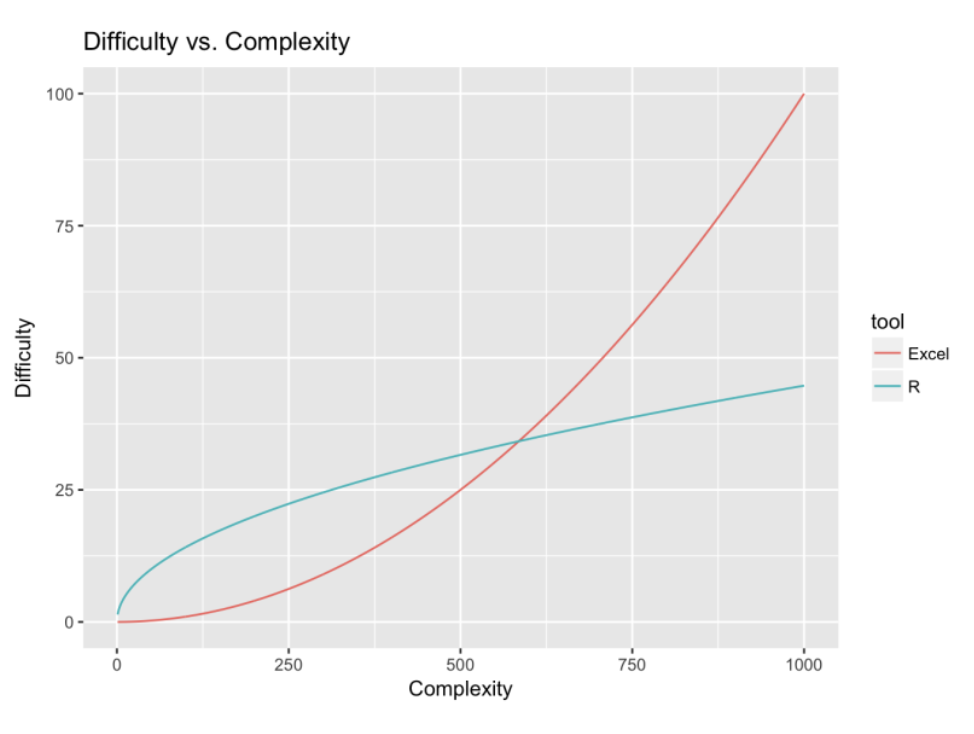
\includegraphics{images/rblogger.png}
Source: R-bloggers

\hypertarget{pourquoi-plus-excel}{%
\subsection{Pourquoi plus Excel ?}\label{pourquoi-plus-excel}}

Un exemple parmi tant d'autres !


\includegraphics{images/covid.png}

Source Alexandre Counis, Les Echos, 5 oct. 2020

\hypertarget{avantages-et-inconvuxe9nients}{%
\section{Avantages et inconvénients}\label{avantages-et-inconvuxe9nients}}

\hypertarget{avantages}{%
\subsection{Avantages}\label{avantages}}

\begin{itemize}
\tightlist
\item
  Souplesse d'utilisation pour réaliser des analyses statistiques
\item
  Libre et gratuit, même s'il existe maintenant des versions payantes de RStudio (shiny et/ou server)
\item
  Reproductibilité des analyses en écrivant/sauvegardant les commandes R dans des scripts
\item
  Large communauté d'utilisateurs/aide en ligne
\item
  Grand nombre de packages spécifiques
\end{itemize}

\hypertarget{inconvuxe9nients}{%
\subsection{Inconvénients}\label{inconvuxe9nients}}

\hypertarget{geeks-and-repetitive-tasks}{%
\section{Geeks and repetitive tasks}\label{geeks-and-repetitive-tasks}}

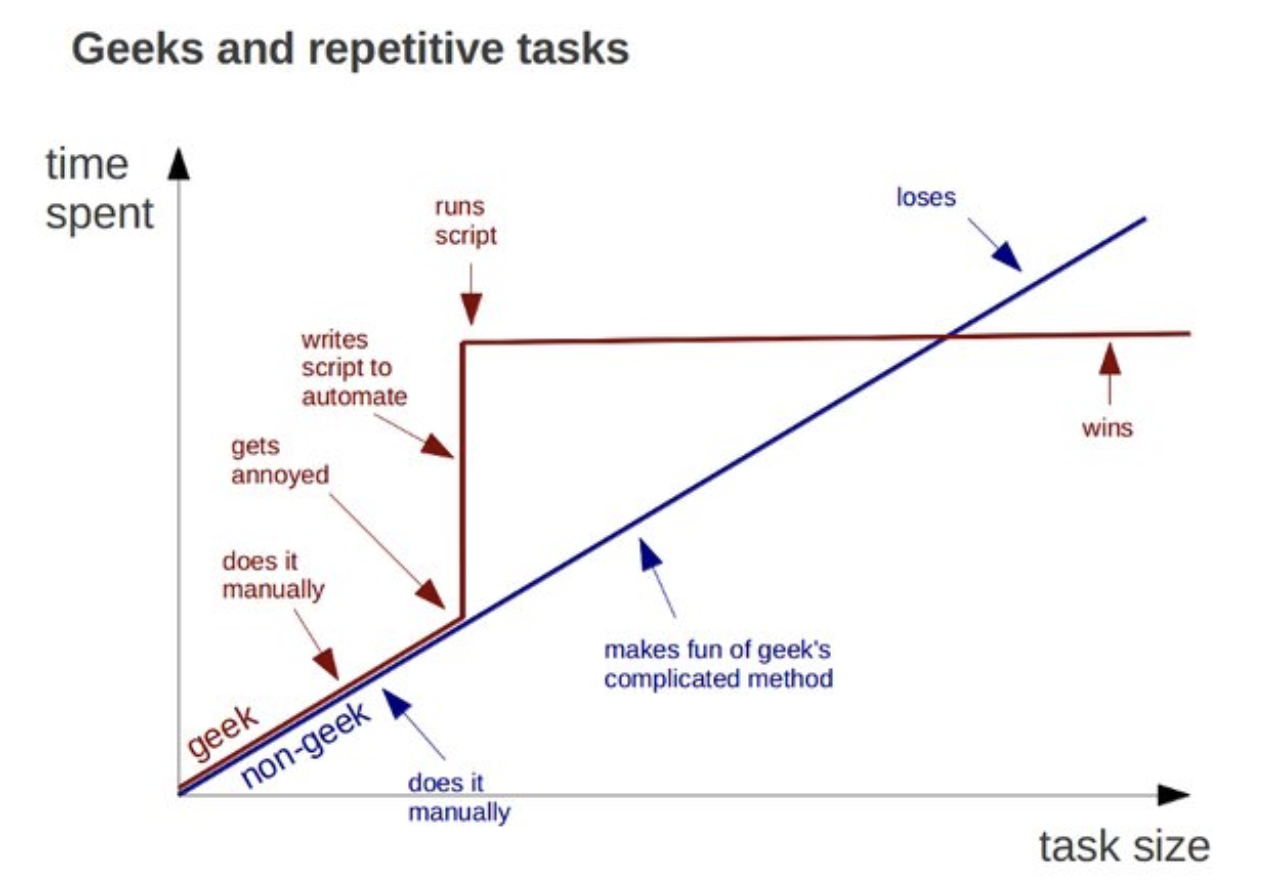
\includegraphics{images/geeks.png}

\hypertarget{r-sait-tout-faire}{%
\section{R sait tout faire}\label{r-sait-tout-faire}}

Lire un tableau de données

\begin{Shaded}
\begin{Highlighting}[]
\FunctionTok{read.table}\NormalTok{()}
\end{Highlighting}
\end{Shaded}

Fusionner deux tableaux

\begin{Shaded}
\begin{Highlighting}[]
\FunctionTok{merge}\NormalTok{()}
\end{Highlighting}
\end{Shaded}

Filtrer des lignes

\begin{Shaded}
\begin{Highlighting}[]
\NormalTok{data[data}\SpecialCharTok{$}\NormalTok{x }\SpecialCharTok{\textgreater{}} \DecValTok{10}\NormalTok{]}
\end{Highlighting}
\end{Shaded}

Sélectionner des colonnes

\begin{Shaded}
\begin{Highlighting}[]
\NormalTok{data[,}\FunctionTok{c}\NormalTok{(“x”,”y”)]}
\end{Highlighting}
\end{Shaded}

Rechercher une chaîne de caractères

\begin{Shaded}
\begin{Highlighting}[]
\FunctionTok{grep}\NormalTok{()}
\end{Highlighting}
\end{Shaded}

Réaliser une ACP

\begin{Shaded}
\begin{Highlighting}[]
\FunctionTok{prcomp}\NormalTok{()}
\end{Highlighting}
\end{Shaded}

Calculer une moyenne

\begin{Shaded}
\begin{Highlighting}[]
\FunctionTok{mean}\NormalTok{()}
\end{Highlighting}
\end{Shaded}

Additionner deux matrices

\begin{Shaded}
\begin{Highlighting}[]
\NormalTok{mat1 }\SpecialCharTok{+}\NormalTok{ mat2}
\end{Highlighting}
\end{Shaded}

Exporter un tableau de données

\begin{Shaded}
\begin{Highlighting}[]
\FunctionTok{write.table}\NormalTok{()}
\end{Highlighting}
\end{Shaded}

Calculer une variance

\begin{Shaded}
\begin{Highlighting}[]
\FunctionTok{var}\NormalTok{()}
\end{Highlighting}
\end{Shaded}

Régression linéaire

\begin{Shaded}
\begin{Highlighting}[]
\FunctionTok{lm}\NormalTok{()}
\end{Highlighting}
\end{Shaded}

Tracer une courbe

\begin{Shaded}
\begin{Highlighting}[]
\FunctionTok{plot}\NormalTok{()}
\end{Highlighting}
\end{Shaded}

Tester une hypothèse

\begin{Shaded}
\begin{Highlighting}[]
\FunctionTok{t.test}\NormalTok{()}
\end{Highlighting}
\end{Shaded}

Dessiner un histogramme

\begin{Shaded}
\begin{Highlighting}[]
\FunctionTok{hist}\NormalTok{()}
\end{Highlighting}
\end{Shaded}

Convertir des données

\begin{Shaded}
\begin{Highlighting}[]
\FunctionTok{as.matrix}\NormalTok{()}
\end{Highlighting}
\end{Shaded}

\hypertarget{comment-utiliser-r}{%
\chapter{Comment utiliser R ?}\label{comment-utiliser-r}}

\hypertarget{modes-dutilisation-liste-non-exhaustive}{%
\section{Modes d'utilisation (liste non exhaustive)}\label{modes-dutilisation-liste-non-exhaustive}}

\begin{itemize}
\tightlist
\item
  Localement via le terminal
\item
  Localement via RStudio (utilisation classique)
\item
  Sur un serveur via le terminal et une connexion ssh
\item
  Sur un serveur via un navigateur web pour accéder à RStudio server
\item
  Sur un serveur via un navigateur web pour accéder à RStudio server par Jupyter
\end{itemize}

\hypertarget{ouverture-ou-connexion-uxe0-rstudio}{%
\section{Ouverture ou connexion à RStudio}\label{ouverture-ou-connexion-uxe0-rstudio}}

3 alternatives :

\begin{enumerate}
\def\labelenumi{\arabic{enumi}.}
\item
  Ouvrir RStudio sur votre propre ordinateur (si installé)
\item
  Vous connecter au serveur Web RStudio de l'IFB
  \url{https://rstudio.cluster.france-bioinformatique.fr}
  puis vous identifier
\end{enumerate}

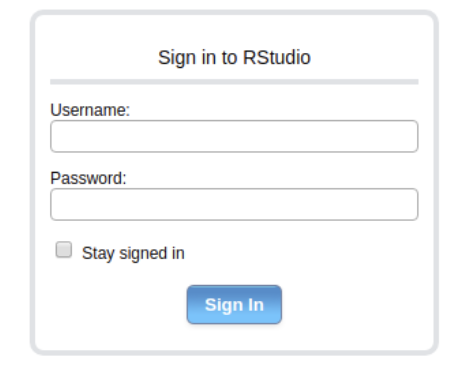
\includegraphics{images/coRstudio.png}

\begin{enumerate}
\def\labelenumi{\arabic{enumi}.}
\setcounter{enumi}{2}
\tightlist
\item
  Vous connecter via Jupyter lab de l'IFB
  \url{https://jupyterhub.cluster.france-bioinformatique.fr}
  puis cliquer sur l'icône RStudio
\end{enumerate}

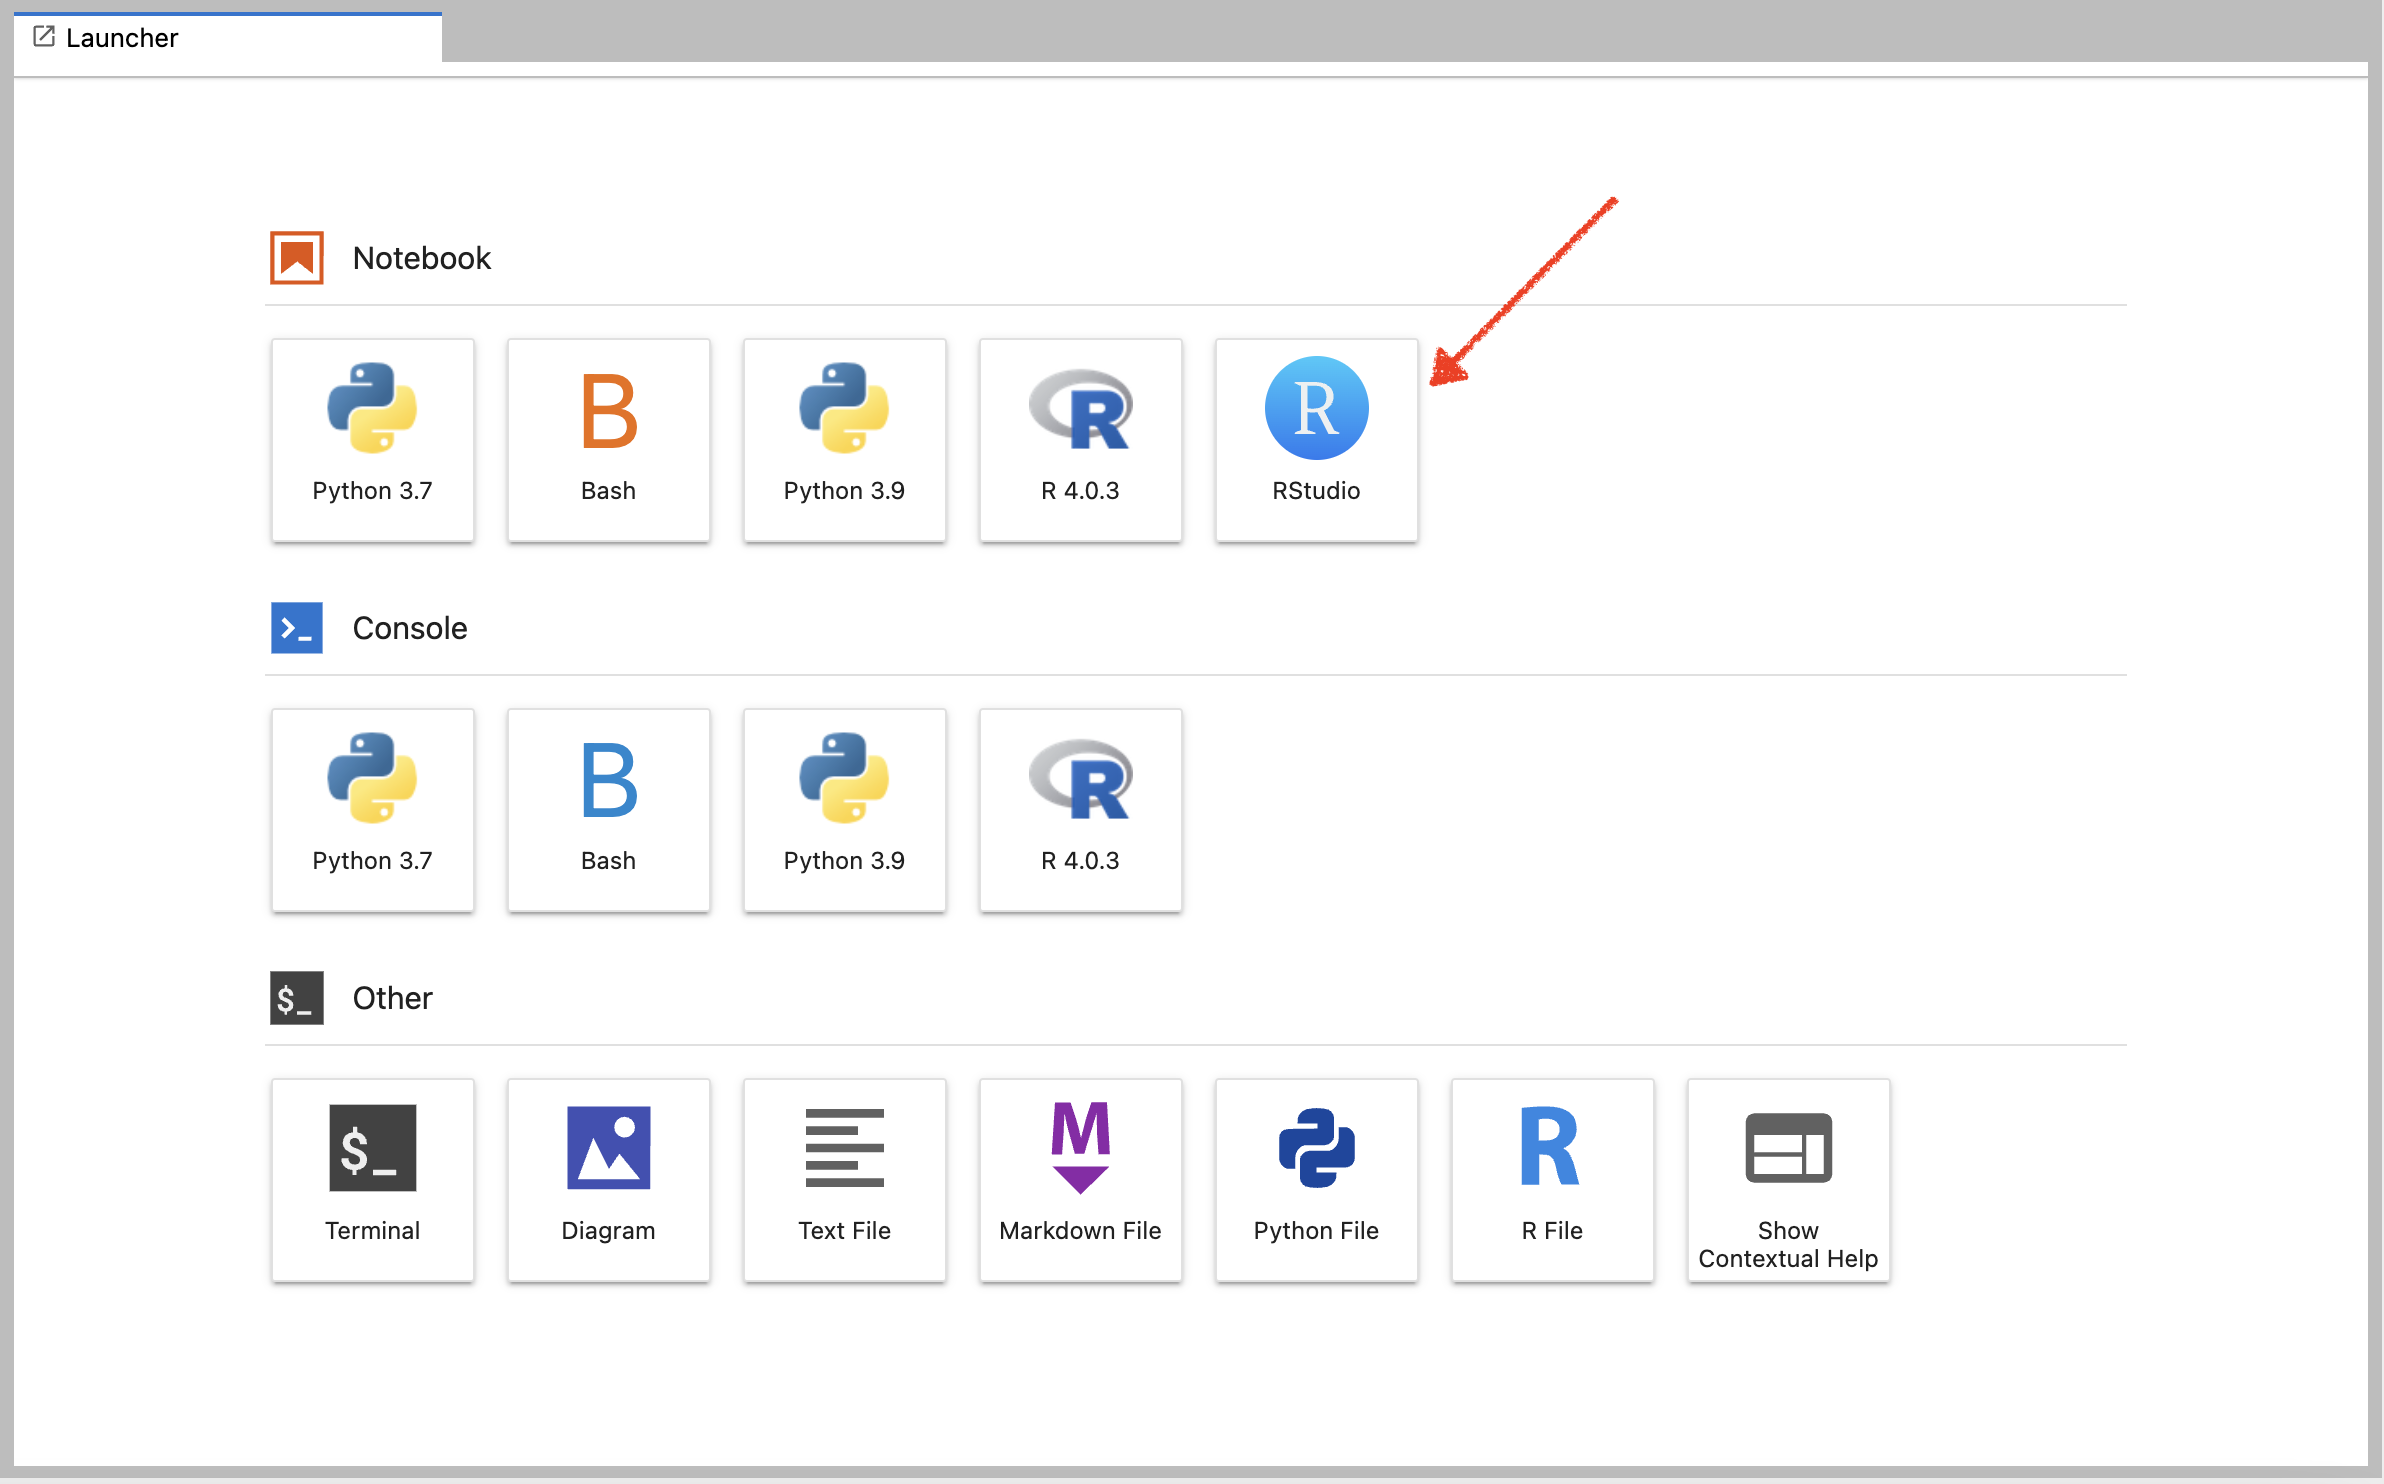
\includegraphics{images/jupyterRstudio.png}

\hypertarget{parts}{%
\chapter{Parts}\label{parts}}

You can add parts to organize one or more book chapters together. Parts can be inserted at the top of an .Rmd file, before the first-level chapter heading in that same file.

Add a numbered part: \texttt{\#\ (PART)\ Act\ one\ \{-\}} (followed by \texttt{\#\ A\ chapter})

Add an unnumbered part: \texttt{\#\ (PART\textbackslash{}*)\ Act\ one\ \{-\}} (followed by \texttt{\#\ A\ chapter})

Add an appendix as a special kind of un-numbered part: \texttt{\#\ (APPENDIX)\ Other\ stuff\ \{-\}} (followed by \texttt{\#\ A\ chapter}). Chapters in an appendix are prepended with letters instead of numbers.

\hypertarget{footnotes-and-citations}{%
\chapter{Footnotes and citations}\label{footnotes-and-citations}}

\hypertarget{footnotes}{%
\section{Footnotes}\label{footnotes}}

Footnotes are put inside the square brackets after a caret \texttt{\^{}{[}{]}}. Like this one \footnote{This is a footnote.}.

\hypertarget{citations}{%
\section{Citations}\label{citations}}

Reference items in your bibliography file(s) using \texttt{@key}.

For example, we are using the \textbf{bookdown} package \citep{R-bookdown} (check out the last code chunk in index.Rmd to see how this citation key was added) in this sample book, which was built on top of R Markdown and \textbf{knitr} \citep{xie2015} (this citation was added manually in an external file book.bib).
Note that the \texttt{.bib} files need to be listed in the index.Rmd with the YAML \texttt{bibliography} key.

The RStudio Visual Markdown Editor can also make it easier to insert citations: \url{https://rstudio.github.io/visual-markdown-editing/\#/citations}

\hypertarget{blocks}{%
\chapter{Blocks}\label{blocks}}

\hypertarget{equations}{%
\section{Equations}\label{equations}}

Here is an equation.

\begin{equation} 
  f\left(k\right) = \binom{n}{k} p^k\left(1-p\right)^{n-k}
  \label{eq:binom}
\end{equation}

You may refer to using \texttt{\textbackslash{}@ref(eq:binom)}, like see Equation \eqref{eq:binom}.

\hypertarget{theorems-and-proofs}{%
\section{Theorems and proofs}\label{theorems-and-proofs}}

Labeled theorems can be referenced in text using \texttt{\textbackslash{}@ref(thm:tri)}, for example, check out this smart theorem \ref{thm:tri}.

\begin{theorem}
\protect\hypertarget{thm:tri}{}\label{thm:tri}For a right triangle, if \(c\) denotes the \emph{length} of the hypotenuse
and \(a\) and \(b\) denote the lengths of the \textbf{other} two sides, we have
\[a^2 + b^2 = c^2\]
\end{theorem}

Read more here \url{https://bookdown.org/yihui/bookdown/markdown-extensions-by-bookdown.html}.

\hypertarget{callout-blocks}{%
\section{Callout blocks}\label{callout-blocks}}

The R Markdown Cookbook provides more help on how to use custom blocks to design your own callouts: \url{https://bookdown.org/yihui/rmarkdown-cookbook/custom-blocks.html}

\hypertarget{sharing-your-book}{%
\chapter{Sharing your book}\label{sharing-your-book}}

\hypertarget{publishing}{%
\section{Publishing}\label{publishing}}

HTML books can be published online, see: \url{https://bookdown.org/yihui/bookdown/publishing.html}

\hypertarget{pages}{%
\section{404 pages}\label{pages}}

By default, users will be directed to a 404 page if they try to access a webpage that cannot be found. If you'd like to customize your 404 page instead of using the default, you may add either a \texttt{\_404.Rmd} or \texttt{\_404.md} file to your project root and use code and/or Markdown syntax.

\hypertarget{metadata-for-sharing}{%
\section{Metadata for sharing}\label{metadata-for-sharing}}

Bookdown HTML books will provide HTML metadata for social sharing on platforms like Twitter, Facebook, and LinkedIn, using information you provide in the \texttt{index.Rmd} YAML. To setup, set the \texttt{url} for your book and the path to your \texttt{cover-image} file. Your book's \texttt{title} and \texttt{description} are also used.

This \texttt{gitbook} uses the same social sharing data across all chapters in your book- all links shared will look the same.

Specify your book's source repository on GitHub using the \texttt{edit} key under the configuration options in the \texttt{\_output.yml} file, which allows users to suggest an edit by linking to a chapter's source file.

Read more about the features of this output format here:

\url{https://pkgs.rstudio.com/bookdown/reference/gitbook.html}

Or use:

\begin{Shaded}
\begin{Highlighting}[]
\NormalTok{?bookdown}\SpecialCharTok{::}\NormalTok{gitbook}
\end{Highlighting}
\end{Shaded}


  \bibliography{book.bib,packages.bib}

\end{document}
